\section{孟德尔遗传}

本章绝大部分内容高中已涉及,故从略,下面只写出高中不涉及的内容。

\subsection{遗传学数据的统计处理}
\subsubsection{组合}

以下内容可参考数学人教A版选择性必修二相关章节。

考虑$Aa$个体自交,$\text{F}_{1}$的基因型比例。一般地,设一种基因型或表型出现的概率为$p$(如在$Aa$自交所得$\text{F}_{1}$中,$Aa$出现的概率为$p=\frac{1}{2}$),且要求$n$个后代中,有$s$个是这种基因型,则这一事件的概率是\[P=\mathrm{C}_{n}^{s}p^{s}(1-p)^{n-s}\]

如$Aa$个体自交所得10个$\text{F}_{1}$中,出现5个$Aa$,4个$aa$,1个$AA$的概率为\[\mathrm{C}_{10}^{5}\times \left ( \frac{1}{2} \right )^{5} \times \mathrm{C}_{5}^{4}\times \left ( \frac{1}{4}  \right )^{4}\times \left ( \frac{1}{4}  \right )  =\frac{315}{8192} \approx 0.038\]

\subsubsection{$\chi^{2}$检验}

对于实际实验所得的数据,大多数情况下并不是完全按照预期比例的\footnote{读者可用组合知识,找个例子计算一下恰好符合比例的概率。},可以用$\chi^{2}$检验来判断所得数据与预期比例是否相符。其公式为:\[\chi^{2}=\sum \frac{\left ( \text{实得数}-\text{预期数} \right ) ^{2}}{\text{预期数} }\quad\text{或写成}\quad \chi^{2}=\sum \frac{\left ( O-E\right ) ^{2}}{E}\]
这里:\begin{itemize}
	\item $O$——Observed,即观察到的“实得数”;
	\item $E$——Expected,即期望得到的“预期数”。
\end{itemize}

计算完$\chi^{2}$后,根据“$\text{自由度df}=\text{分类数}-1$”查$\chi^{2}$表(\autoref{tab:chisq_table}为$\chi^{2}$表的一部分),得到$P$的范围,若$P<0.05$,则表明符合预期比例。需要指出的是,$\chi^{2}$检验仅是一种估计值,在样本数小于5时,建议使用组合法估计概率。

\begin{table}[h!]
	\centering
	\begin{tabular}{|c|c|c|c|c|}
		\hline
		\multirow{2}{*}{自由度df} & \multicolumn{4}{c|}{概率$P$} \\ \cline{2-5}
		& 0.10   & 0.05   & 0.01   & 0.001  \\ \hline
		1                                        & 2.706 & 3.841 & 6.635 & 10.828 \\ \hline
		2                                        & 4.605 & 5.991 & 9.210 & 13.816 \\ \hline
		3                                        & 6.251 & 7.815 & 11.345& 16.266 \\ \hline
		4                                        & 7.779 & 9.488 & 13.277& 18.467 \\ \hline
		5                                        & 9.236 & 11.070& 15.086& 20.515 \\ \hline
	\end{tabular}
	\caption{$\chi^{2}$表}
	\label{tab:chisq_table}
\end{table}

在$\chi^{2}$表中,表内数字是各种$\chi^{2}$值,$P$表示在一定自由度下,$\chi^{2}$大于表中数值的概率。


\subsection{孟德尔遗传病}

常见的孟德尔遗传病在\autoref{tab:OMIM}中已经列出。

\begin{gs}[:红绿色盲的遗传]
	有这么一位女孩,她在学校里总是得过且过,对学习毫无用心。在一次考试中,她仅得10分,老师用红笔在试卷上写下了分数,并要求家长在试卷上签字。于是,女孩心生一计,想给父亲一个“惊喜”。她偷偷在分数后面添了一个“0”,将10分篡改为100分。随后,她将试卷交给了父亲。父亲接过试卷,瞬间暴怒:“你这100分的最后一个‘0’怎么是绿色的?你以为我是傻子吗?暂且不说你只考了10分就敢篡改成绩,你连改成绩都不会改?”过了一会儿,父亲突然明白了什么。请问:父亲知道了什么?
\end{gs}
\newpage
\begin{table}[htbp]
	\centering
	\begin{tabularx}{\textwidth}{|c|X|}
		\hline
		\multicolumn{1}{|l|}{遗传方式} & \multicolumn{1}{c|}{疾病}                                     \\ \hline
		\multirow{3}{*}{常显}        & 亨廷顿舞蹈病(HD):致病基因\textit{HTT}内部CAG三核苷酸串联重复,重复数越多,发病越早、症状越重。   \\ \cline{2-2}
		& 马方综合征                                                       \\ \cline{2-2}
		& 多指/趾症                                                       \\ \hline
		\multirow{4}{*}{常隐}        & 囊性纤维化(CF):位于7q\footnotemark 的致病基因常发生三核苷酸非移码的缺失,导致CFTR这种氯离子通道蛋白508号位Phe缺失。 \\ \cline{2-2}
		& 半乳糖血症                                                       \\ \cline{2-2}
		& 苯丙酮尿症                                                       \\ \cline{2-2}
		& 白化病                                                         \\ \hline
		\multirow{3}{*}{X显}        & 抗维生素D佝偻病:肾小管遗传性缺陷,致病基因\textit{PHEX}位于Xp。                    \\ \cline{2-2}
		& 遗传性肾炎                                                       \\ \cline{2-2}
		& 色素失调症                                                       \\ \hline
		\multirow{3}{*}{X隐}        & 血友病:甲型由于凝血因子VIII缺陷,乙型由于凝血因子IX缺陷,都定位于Xq。                     \\ \cline{2-2}
		& 蚕豆病(6-磷酸葡萄糖脱氢酶缺乏症)                                            \\ \cline{2-2}
		& 红绿色盲                                                        \\ \hline
	\end{tabularx}
	\caption{常见孟德尔遗传病}
	\label{tab:OMIM}
\end{table}
\footnotetext{关于染色体上具体位置的表示方法见后文。}
\subsection{孟德尔遗传的拓展}

许多性状并不能完美地用孟德尔遗传规律解释,这是因为表型受到环境和其他基因的影响。

\subsubsection{环境对表型的影响}

基因型相同,表型可能不同;基因型不同,表型可能相同。环境可以指生物体以外的环境,也可以指其他基因的影响。生物体的基因型是生物发育的内因,表型是环境和基因型共同作用的结果。

\subsubsection{性状的多基因决定}

多个基因可以共同决定一个性状。

\subsubsection{基因的多效性}

一个基因可以决定多个性状,这是因为生物体内各种生理生化过程都是相互联系和制约的。

\subsubsection{表现度和外显率}

表现度指的是在具有相同基因型的个体间,基因表达的变化程度。这类似于模拟信号0\textasciitilde1的变化。外显率指的是在所有具有一种基因型的个体中,表现出这种表型的个体比例。这类似于数字信号0或1的区别。

\subsubsection{拟表型(表型模写)}

环境导致的表型变化,就如同某基因改变引起了这种变化一样,这叫做表型模写。

\subsection{显隐性的相对性}

在一些情况下,显性是不完全的(即\textit{Aa}和\textit{AA}表型不同),或显隐性可根据所需标准更改。

\subsubsection{不完全显性}

杂合子中显性性状不能完全掩盖隐性性状的现象称为不完全显性,杂合子的性状介于纯合双亲之间。如黑缟蚕和白蚕杂交后代为淡黑缟蚕。杂合子\textit{Aa}自交后代分离比是$1:2:1$。

\subsubsection{镶嵌显性}

镶嵌显性的的基因,杂合子在不同部位分别表现双亲的性状,如瓢虫鞘翅色斑。
\subsubsection{共显性}

共显性遗传的基因,杂合子在同一部位表现出双亲的性状。一个例子是MN血型,其等位基因为$L^{M}$和$L^{N}$。

\subsubsection{显隐性可随所依据的标准更改}

基因的显隐性关系其实只是人为附加的,所采用的标准不同,显隐性可能不同。下面表格(\autoref{tab:relativeDominance})以镰状细胞贫血这一孟德尔疾病为例来说明。镰状细胞贫血有两个等位基因:$HBB^{A}$与$HBB^{s}$。
\begin{table}[h!]
	\centering
	\begin{tabularx}{\textwidth}{|c|c|c|c|X|}
		\hline
		认为的显性性状 & $HBB^{A}HBB^{A}$ & $HBB^{A}HBB^{s}$ & $HBB^{s}HBB^{s}$ & \multicolumn{1}{c|}{显隐性关系} \\ \hline
		健康无症状   & 是                & 是                & 否                & $HBB^{A}$对$HBB^{s}$为显性     \\ \hline
		红细胞呈镰状  & 否                & 部分               & 是                & $HBB^{s}$对$HBB^{A}$为不完全显性  \\ \hline
	\end{tabularx}
	\caption{显隐性的相对性}
	\label{tab:relativeDominance}
\end{table}

\subsubsection{显隐性关系与环境}

即使所依据的标准不变,显隐性关系还可能随环境而变——包括内环境和外部环境。如曼陀罗的紫茎和绿茎是一对相对性状,夏季杂合子为紫茎,但温度较低时,杂合子茎的紫色就变浅,紫色已不是完全显性的了。

又如一种牛,毛被的红褐色与红色是一对相对性状,杂合子的表型与性别有关。雄牛是红褐色,雌牛是红色,这可能是性激素影响的结果。像这样,相同基因型的不同性别个体,表型不同的现象叫做\sy{从性遗传}。

\subsection{致死基因}

有的基因处于杂合或纯合状态时会导致个体死亡,这叫致死基因。纯合致死的例子有:黄色小鼠、镰状细胞贫血、植物的白化基因。杂合致死,也就是显性致死的例子是人的结节性硬化症(TS)。

\subsubsection{致死的时期}

致死作用可发生在不同的发育阶段,在配子期致死的为\sy{配子致死},在胚胎期或成体阶段致死的为\sy{合子致死}。致死的效果也不总是$100\%$的,\sy{亚致死现象}的致死率可在0\textasciitilde100\%之间变动。

\subsubsection{环境的影响}

致死基因的作用同样可受到环境影响。有的基因型在几乎所有环境都致死,而有的在特别的环境则可以生活。如选育出的花卉,精心培育可以生活,而当它在野外则无法生存。

\subsection{复等位现象}

前述的等位基因都只有两个,如\textit{A}和\textit{a}。其实一个基因可以有很多等位形式,像$a_{1},a_{2},a_{3}$……这样。这叫做\sy{复等位基因}。下面是一些实例。

\subsubsection{瓢虫的鞘翅色斑}

这东西实在无聊,略。

\subsubsection{孟买型、ABO血型}

合成红细胞表面H物质的基因为显性\textit{H},这是A、B抗原的共同前体,则\textit{hh}个体(即\sy{孟买型})因无法合成H物质,表现出O型\footnote{由此可见,\textit{h}对$I^{A}$、$I^{B}$是隐性上位关系。这将在后面详述。}。

\begin{table}[h!]
	\centering
	\begin{tabular}{|c|c||c|c|}
		\hline
		基因型          & 血型(表型)             & 基因型          & 血型(表型)             \\ \hline
		$I^{A}I^{B}$ & AB                 & $I^{B}i$     & \multirow{2}{*}{B} \\ \cline{1-3}
		$I^{A}i$     & \multirow{2}{*}{A} & $I^{B}I^{B}$ &                    \\ \cline{1-1} \cline{3-4}
		$I^{A}I^{A}$ &                    & $ii$         & O                  \\ \hline
	\end{tabular}
	\caption{ABO血型与基因型的关系}
	\label{tab:ABObloodType}
\end{table}

\subsubsection{Rh血型与母子不相容}

Rh血型由\textit{R}和\textit{r}基因决定,\textit{RR}和\textit{Rr}都是Rh阳性,红细胞膜表面有相关抗原;\textit{rr}个体为Rh阴性,无抗原,二者体内自然状态下都无该种抗原的抗体。我国大多数人都是Rh阳性。

对于Rh抗原,更严谨的说法是,它包含抗原性从强到弱D、E、c、C、e五种抗原。Rh阳性或阴性即有无D抗原。
\subsubsection{人类的母子不相容}

Rh阴性的母亲分娩Rh阳性第一胎时,胎儿Rh阳性红细胞可能进入母亲体内,最终导致产生抗体。该母亲怀第二胎若也是Rh阳性,由于胎盘对抗体通透,故抗体将进入胎儿血液,导致胎儿死亡,即使存活,也患有新生儿溶血症。第一胎并不会患病,因为抗体是在分娩后才产生的。

实际上,上述情况并不多见,因为:
\begin{itemize}
	\item 有些产妇并不会产生这种抗体;
	\item Rh抗原并非水溶性,只有Rh阳性红细胞进入母亲血液才有机会发生免疫反应;
	\item 如父亲是\textit{Rr},则只有$50\%$生下Rh阳性儿;
	\item 第一胎的红细胞可因其他血型的不相容而避免发生免疫反应,如A型红细胞被母亲血液中的A抗体破坏。
\end{itemize}

对于产下Rh阳性第一胎的Rh阴性产妇,可在分娩后肌肉注射Rh抗体,在自身产生免疫反应之前把Rh阳性红细胞破坏。等到这抗体浓度下降后,可以怀第二胎Rh阳性儿。如果是第二胎已经分娩,那只能采取换血的治疗方法。

\subsubsection{家畜的母子不相容}

母马和公驴杂交产生的骡,有时也出现溶血。不过,母畜产生的抗体并非从胎盘传递给骡驹,而是通过母乳。所以,只需要弃用抗体效价高的初乳,先人工哺乳,过段时间再自由哺乳即可。而对于已经患病的骡驹,可以输合适的马血治疗。

\subsubsection{自交不亲和}

暂时从略,参见植物生理。

\subsection{非等位基因间的相互作用}

\subsubsection{互补基因}

两对非等位基因相互作用,出现了新的性状,这两对基因就叫互补基因。如我们熟悉的孟德尔豌豆的$Y/y$与$R/r$。另外还有香豌豆花冠颜色的遗传,也是互补基因。这是\textit{C}和\textit{R}相互作用的结果。

\subsubsection{修饰基因}

修饰基因自己没有表型效应,它存在时通过影响其他基因来影响表型,这叫做。按作用分为:
\begin{itemize}
	\item 强化基因——加强其他基因的表型效应;
	\item 限制基因——减弱其他基因的表型效应;
	\item 抑制基因——完全抑制其他基因的表型效应。
\end{itemize}

例如:

\subsubsection{上位效应}

上位基因有自己的表型,当它处于显性或隐性纯合状态时,可以抑制其他非等位基因的表性效应。这种作用分别称为显性上位或隐性上位。

\section{分子遗传}

\subsubsection{粗糙链孢霉的生化突变型}

在生物体内,精氨酸的合成代谢途径是:
\begin{center}
	\textit{N}-乙酰瓜氨酸$\longrightarrow$鸟氨酸$\longrightarrow$瓜氨酸$\longrightarrow$精氨酸
\end{center}

在精氨酸缺陷型粗糙链孢霉培养基中分别加入鸟氨酸、瓜氨酸、精氨酸,生长情况如\autoref{tab:arginineDeficientRoughMutantOfNeurosporaCrassaExperimentalResults}所示。

\begin{table}[htbp]
	\centering
	\begin{tabularx}{\textwidth}{|c|C|C|C|}
		\hline
		& 鸟氨酸 & 瓜氨酸 & 精氨酸 \\ \hline
		$arg_3$ & --- & --- & + \\ \hline
		$arg_2$ & --- & + & + \\ \hline
		$arg_1$ & + & + & + \\ \hline
	\end{tabularx}
	\caption{精氨酸缺陷型粗糙链孢霉实验结果}
	\label{tab:arginineDeficientRoughMutantOfNeurosporaCrassaExperimentalResults}
\end{table}

从“---”数目最多的那一个菌株看起,表明该菌株缺乏直接合成精氨酸的酶。其余菌株缺少的酶,按照“---”数目递减,向前推即可。

由此可知,催化精氨酸合成反应的酶应分别对应于下面步骤:
\begin{center}
	\textit{N}-乙酰瓜氨酸$\xrightarrow{arg_1}$鸟氨酸$\xrightarrow{arg_2}$瓜氨酸$\xrightarrow{arg_3}$精氨酸
\end{center}

\subsection{人的先天代谢缺陷}

\subsubsection{苯丙酮尿症、白化病、尿黑酸症}

苯丙酮尿症、白化病、尿黑酸症的发病原理如\autoref{fig:phe_pathway}:

\begin{figure}[htbp]
	\centering
	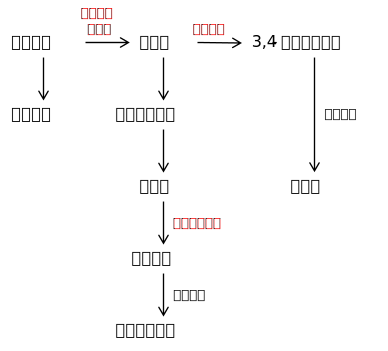
\includegraphics{苯丙氨酸代谢疾病.pdf}
	\caption{苯丙氨酸代谢途径}
	\label{fig:phe_pathway}
\end{figure}

这三种疾病鳄基因都是隐性基因,缺陷的酶用{\color[RGB]{255,0,0}红色}标出。
\begin{itemize}
	\item 苯丙酮尿症患者不能把苯丙氨酸转化为酪氨酸,故苯丙氨酸积累,可损害中枢神经系统,影响智力发育。因为酪氨酸不可自己合成,只能依靠食物,故黑色素缺乏。
	\item 白化病患者缺乏酪氨酸酶,无法合成黑色素。
	\item 尿黑酸症患者不能形成尿黑酸氧化酶,因此不能继续转变的尿黑酸只好进入尿液,在空气中被氧化后,就从无色变为黑色。
\end{itemize}

\subsubsection{半乳糖血症}

极少数婴儿缺乏1-磷酸葡糖尿苷转移酶(如\autoref{fig:banrutang_tujing}所示红色{\color[RGB]{255,0,0}酶}字,另见\autopageref{fig:leloir}的\autoref{fig:leloir}),无法利用半乳糖。症状严重,可致婴儿死亡。但可以通过控制饮食来避免摄入半乳糖,生长发育就	相当正常。

\begin{figure}[htbp]
	\centering
	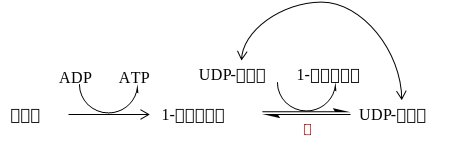
\includegraphics{半乳糖代谢.pdf}
	\caption{半乳糖的代谢途径}
	\label{fig:banrutang_tujing}
\end{figure}

\subsection{位置效应}

基因的位置效应即:基因的不同位置,对表型有影响。

\subsection{顺反子}



\section{性别决定}

一般的性别决定方式是依靠性染色体(XY或ZW),也有取决于染色体组数或环境的。

\subsection{常见的性别决定}

\subsubsection{XY型性别决定}

最常见的一种性别决定方式。全部哺乳动物、大多数昆虫(包括果蝇)、很多雌雄异株植物都是XY性别决定。同配(XX)为雌性,异配(XY)为雄性。

\subsubsection{ZW型性别决定}

实例有家蚕、鸟、多数鳞翅目昆虫。同配(ZZ)为雄性,异配(ZW)为雌性。

\subsection{特殊的性别决定}

\subsubsection{蜂的性别决定}

蜂的性别由染色体倍性决定。单倍体为雄性,二倍体为雌性。雄峰通过假减数分裂产生配子。假减数分裂时形成的纺锤体为单极纺锤体。

\subsubsection{后螠的性别决定}

后螠的雌虫大,雄虫小。雄虫生活在雌虫的子宫内。自由游泳的幼虫是中性的。若:

\begin{description}
	\item[落在海底] 成为雌虫;
	\item[落在雌虫口吻上] 成为雄虫。
\end{description}

\subsubsection{高等植物的性别决定}

高等植物由染色体上的基因决定性别。

\subsection{环境对决定的影响}

\subsubsection{温度}

某些动物的卵在不同温度,发育出的幼体性别不同。

\begin{description}
	\item[高温为雄性,低温为雌性] 鳄鱼、短吻鳄、蜥蜴、蝾螈等。
	\item[高温为雌性,低温为雄性] 常见的就是海龟。
\end{description}

\subsubsection{激素}

牛一胎生下雌雄两犊时,雌性不育而雄性正常。雌性性腺像雄性的。原因是:
\begin{itemize}
	\item 在胚胎期,雄性的性腺先发育,雄激素通过胎盘进入雌性体内;
	\item 细胞也会进入对方体内,Y染色体有雄性化作用。
\end{itemize}

雌鸡的性逆转也与激素有关。

\subsubsection{日照}

大麻的性别受日照长度的影响。

\subsection{人类的性别决定}

\subsubsection{睾丸决定因子}

人类的性别由Y染色体决定,无Y染色体的个体发育成雌性,有Y染色体的发育为雄性。

Y染色体上的睾丸决定因子最为关键。睾丸决定因子即\textit{SRY}基因,编码转录因子。由于\textit{SRY}所在区域与XY之间的拟常染色体区靠近,故可能发生交换,形成无\textit{SRY}的Y染色体和含\textit{SRY}的X染色体。

雄性性别的形成还涉及到SRY下游一系列信号,当相关基因异常,也无法发育为雄性。雄性性别的形成也有常染色体的功劳。

\subsubsection{性指数}

果蝇的性别由X染色体和常染色体的倍数比值(X:A)决定(\autoref{tab:果蝇性别与性指数的关系}),而Y染色体存在与否决定果蝇的育性。X:A即性指数。

\begin{table}[htbp]
	\begin{tabularx}{\textwidth}{|C|C|}
		\hline
		X:A & 性别 \\ \hline
		$\geq$1.0 & 雌性 \\ \hline
		$\leq$0.5 & 雄性 \\ \hline
		0.5\textasciitilde1之间 & 中间性(发育异常) \\ \hline
	\end{tabularx}
	\caption{果蝇性别与性指数的关系}
	\label{tab:果蝇性别与性指数的关系}
\end{table}



\section{连锁分析}

\subsection{连锁与交换}

\subsection{普通连锁分析}

\subsection{粗糙链孢霉的连锁分析}

\section{细菌和噬菌体的重组和连锁}

\subsection{细菌和噬菌体遗传分析的特点}

细菌是单倍体,不发生减数分裂。细菌个体之间存在基因转移和重组。细菌中,遗传物质传递的方式有:转化、接合、转导。

不同基因型的噬菌体混合侵染细菌时,可发生两个基因组之间的同源重组。

\subsection{噬菌体的连锁分析}

对细菌进行\sy{双重感染(混合感染)},即用两种基因型的噬菌体侵染细菌,将子代噬菌体接种在有菌株的培养基上。则两基因的重组率:\[\text{重组率}=\frac{\text{重组噬菌斑数}}{\text{总噬菌斑数}}\]

\subsection{细菌的连锁分析}

\subsubsection{F$^{+}$、F′、Hfr、F$^{-}$菌株}

\begin{description}
	\item[F$^{+}$菌株] 具有F因子(F质粒),菌体表面有性伞毛。可长出接合管把F质粒复制一份后,传递给F$^{-}$菌株,F$^{-}$菌株拥有了F质粒就变成F$^{+}$。但是细菌基因组转移率很低。
	\item[Hfr菌株] F因子与细菌基因组环状DNA发生一次交换,使F因子整合进细菌基因组。Hfr菌株能高频转移细菌基因组到F$^{-}$菌中,但由于F质粒基因比较靠后,所以F因子很少转移。
	\item[F′菌株] F′菌的F因子含有部分细菌基因组DNA。这是由于Hfr的F因子整合进细菌基因组后,携带少量细菌基因组,再脱离出来。
	\item[F$^{-}$菌株] 不具有F因子。
\end{description}

归纳如\autoref{tab:hfr_fff}:

\begin{table}[htbp]
	\centering
	\begin{tabularx}{\textwidth}{|c|C|C|C|}
		\hline
		\textbf{菌株} & \textbf{F因子} & \textbf{F因子转移} & \textbf{基因组转移} \\ \hline
		F$^{+}$ & 有 & 是 & 否 \\ \hline
		F′ & 有,含部分基因组 & 是 & 仅F因子上的 \\ \hline
		Hfr & 有,在基因组上 & 低频 & 高频 \\ \hline
		F$^{-}$ & 无 & --- & --- \\ \hline
	\end{tabularx}
	\caption{F$^{+}$、F′、Hfr、F$^{-}$菌株的比较}
	\label{tab:hfr_fff}
\end{table}

\subsubsection{转化及作图}

\subsubsection{接合及作图}

\subsubsection{中断杂交作图}

\subsubsection{重组作图}

\subsubsection{转导}


\section{数量性状遗传}

性状有质量性状和数量性状之分。\sy{质量性状}即不连续差异,如水稻的\xpinyin*{粳}、糯,人的ABO血型等。\sy{数量性状}即连续的、界限不清晰的性状区别,如奶牛泌乳量、人的智商、棉花纤维长度等。

\subsection{数量性状的遗传分析}

多基因假说认为,每一个数量性状都是许多基因共同作用的结果。其中每一个基因作用效果较小,与环境造成的差异差不多,所以基因型不同造成的表性差异看起来就是连续的了。

\subsection{分析数量性状的基本统计学方法}

\subsection{遗传率}

\subsection{近交系数和亲缘系数}

\section{遗传物质的改变}

\subsection{染色体结构改变}

\subsubsection{研究方法}

\subsubsection{缺失}

\subsubsection{重复}

\subsubsection{倒位}

\subsubsection{易位}

\subsection{染色体数目改变}

\subsection{基因突变}

\section{细胞质和遗传的关系}

\subsection{母性影响}

\subsection{细胞质遗传}

\subsection{核质互作与禾谷类作物雄性不育}



\section{基因组}

\section{遗传分析}

\section{遗传与个体发育}

